\chapter{Rilascio}
\label{chap:rilascio}
In questa sezione viene presentato il rilascio del prodotto finale, presentando infine un esemptio di integrazione dell'SDK
all'interno di un prodotto Datasoil S.rl. operativo.

\section{Rilascio SDK}
Al fine di rilasciare un package, è necessario effettuare la \textit{build} del prodotto. \\
Per il processo di building del codice è stato utilizzato \textit{Rollup}, un bundler di moduli JavaScript che permette:
\begin{itemize}
    \item di creare bundle di moduli in formato \textit{ESM} (ECMAScript Module) e \textit{CJS} (CommonJS);
    \item di utilizzare TypeScript all'interno del progetto, integrando la configurazione dichiarata nel file \textit{tsconfig.json};
    \item la risoluzione delle dipendenze tra i moduli, escludendo le \textit{peerdependency} dal bundle;
    \item la produzione di bundle di dimensioni ridotte grazie alla sua capacità di effettuare il tree-shaking;
    \item il supporto al plugin \textit{terser}, utilizzato per la minimizzazione del codice prodotto attraverso la rimozione dei commenti e degli spazi vuoti,
          effettuando il \textit{munging} dei nomi delle variabili e introducendo ottimizzazioni per ridurre la dimensione finale;
    \item il supportare a \textit{sourcemaps} per facilitare il debug del codice, permettendo di mappare il codice minificato con il codice sorgente originale;
    \item la generazione di file di dichiarazione TypeScript;
    \item il supporto a plugin per il calcolo della dimensione del bundle, specificando la dimensione di ogni singola dipendenze
          all'interno del progetto, generando un file di report \textit{html}.
\end{itemize}
Per effettuare la build del progetto è necessario eseguire il comando \textit{yarn build-package} configurato all'interno del file \textit{package.json} del progetto:
tale comando, come mostrato nel listato \ref{listing:scripts_package_json_dsdashboard2}, effettua la build del progetto, generando i file di output all'interno della cartella \textit{dist}.\\
Data la configurazione all'interno del file \textit{rollup.config.js}, il comando effettua la build del progetto in formato \textit{ESM} e \textit{CJS}.\\
Per specificare il punto di ingresso per i consumatori dei package, sono state definite all'interno del file \textit{package.json} le chiavi \textit{main} e \textit{module} che puntano
rispettivamente ai file \textit{dist/cjs/index.js} e \textit{dist/esm/index.esm.js}.
Utilizzando \textit{Yarn}, il rilascio di un package può avvenire principalmente tramite tre modalità differenti:
\begin{itemize}
    \item \textbf{Registro di npm}: è il registro di default di \textit{Yarn}, un registro pubblico che permette a chiunque abbiano
          un account di pubblicare pacchetti. Per impostazione predefinita (ma comunque configurabile), i pacchetti pubblicati su \textit{npm}
          sono visibili a tutti e di conseguenza tutti possono usufruirne;
    \item \textbf{Registro privato}: è un registro privato che permette di pubblicare pacchetti in un ambiente accessibile solo a chi è
          autorizzato. Esistono differenti servizi che offrono registri privati, a seconda del contesto operativo e delle esigenze dei prodotti
          che devono usufruire di tali pacchetti;
    \item \textbf{Github Packages}: è un \textit{software package hosting service} offerto da \textit{Github} che permette di pubblicare pacchetti
          in modo pubblico o privato all'interno di un repository \textit{Github}, come se fosse un registro \textit{npm}.
\end{itemize}
Per questo progetto è stato scelto di utilizzare quest'ultima opzione come registro di pubblicazione dei pacchetti, in quanto
all'interno di Datsoil S.r.l. i package prodotti vengono pubblicati all'interno dello spazio \textit{Github Packages} dell'organizzazione aziendale:
questo servizio è infatti molto utile per chi utilizza \textit{Github} come sistema di versionamento e vuole mantenere i pacchetti all'interno del proprio repository.
Per pubblicare un pacchetto all'interno di \textit{Github Packages} è necessario configurare il file \textit{package.json} del progetto, specificando
il campo \textit{publishConfig} nel seguente modo:

\begin{listing}[H]
    \begin{minted}{json}
    {
        "publishConfig": {
            "registry": "https://npm.pkg.github.com/"
        }
    }
    \end{minted}
    \caption{Configurazione del campo \textit{publishConfig} all'interno del file \textit{package.json}}
    \label{listing:package_json_publish_config}
\end{listing}

In seguito, dopo aver configurato il file \textit{.npmrc} all'interno del progetto, specificando il token di autenticazione per l'accesso al registro di \textit{Github Packages},
è possibile eseguire il comando \textit{yarn publish} per pubblicare il pacchetto: una volta avviato il comando, verrà illustrata la versione precedente del
package e verrà richiesto di fornirne una nuova. \\
Una volta terminato il processo di pubblicazione, il pacchetto sarà disponibile all'interno del registro di \textit{Github Packages} dell'organizzazione aziendale.

\section{Integrazione SDK all'interno di SYNMGR}
Durante lo svolgimento dello stage, ho avuto la possibilità di integrare l'SDK prodotto all'interno del prodotto \textit{SYNMGR} di Datasoil S.r.l.,
applicazione web di test utilizzata dall'azienda per testare gli sviluppi futuri e le nuove funzionalità che verranno in seguito rilasciate sul prodotto ufficiale \textit{SYN}. \\
Per utilizzare l'SDK all'interno di \textit{SYNMGR}, è stato necessario configurare il file \textit{.npmrc} all'interno del progetto, specificando il token di autenticazione
per l'accesso al registro di \textit{Github Packages}: utilizzando infatti il registro fornito da \textit{Github}, i package manager come \textit{Yarn} e \textit{npm} andranno
a verificare la presenza di tali informazioni e, solo nel caso di riscontro positivo, permetteranno l'installazione dei pacchetti. \\
In seguito, è stata sostituito il precedente SDK \textit{dsdashboard} a favore del nuovo SDK \textit{dsdashboard2} all'interno del file \textit{package.json} del progetto.

\begin{listing}[H]
    \begin{minted}{json}
    {
        "dependencies": {
            "@datasoil/dsdashboard2": "^0.1.5"
        }
    }
    \end{minted}
    \caption{Configurazione del campo \textit{dependencies} all'interno del file \textit{package.json} di \textit{SYNMGR}}
    \label{listing:package_json_synmgr}
\end{listing}

In seguito, è stato eseguito il comando \textit{yarn install} per installare il pacchetto all'interno del progetto, permettendo di utilizzare le nuove implementazioni delle
componenti inerenti alle dashboard.

\begin{figure}[H]
    \centering
    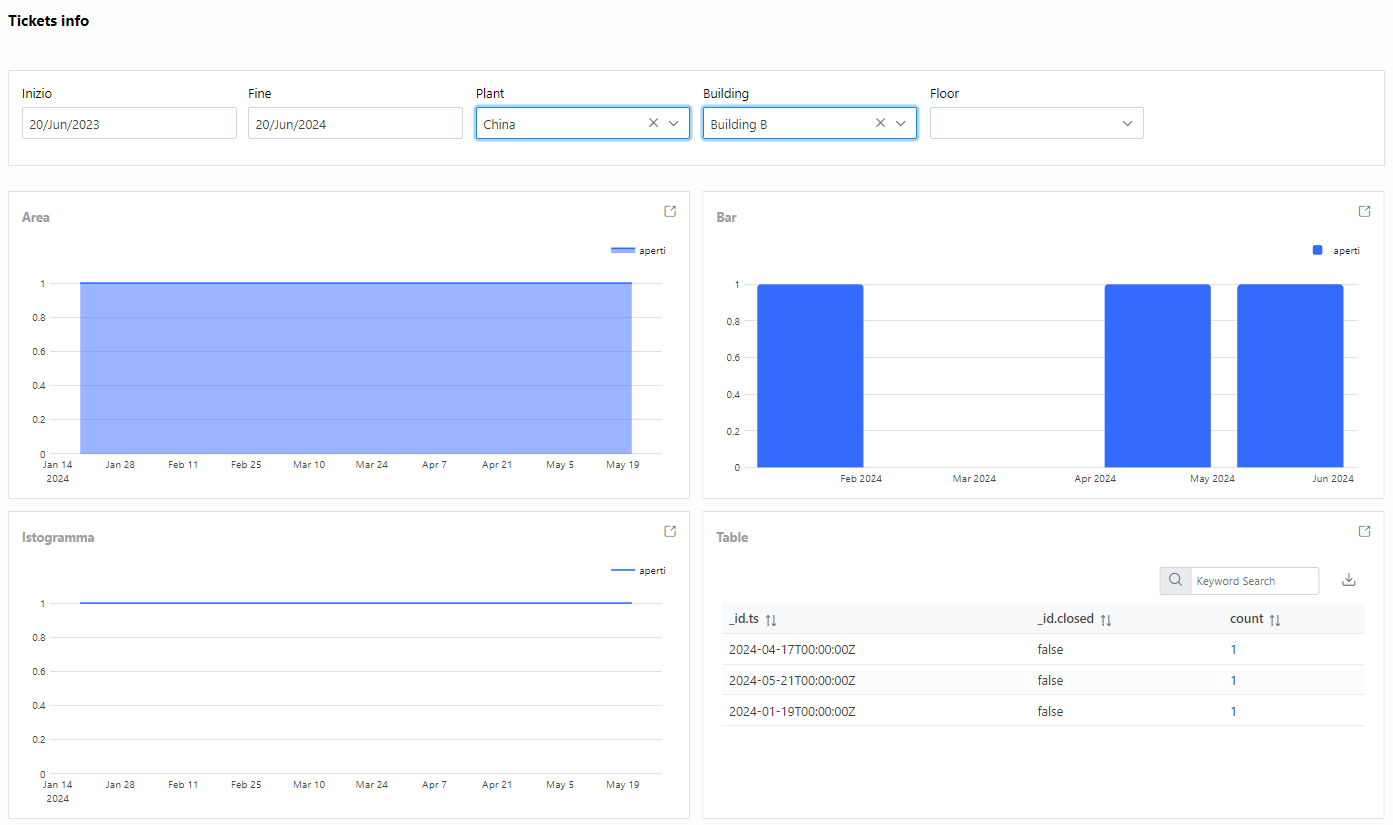
\includegraphics[alt={Esempio di dashboard all'interno di SYNMGR}, width=1 \columnwidth]{img/synmgr-dashboard.png}
    \caption{Esempio di dashboard all'interno di SYNMGR}
    \label{fig:synmgr_dashboard}
\end{figure}